\chapter{La cryptographie à travers l'histoire}
Avant de commencer à décrire la cryptographie en soit, voyons un peu
son histoire, son apparition, et son évolution au fil du temps.

\section{L'apparition de la cryptographie}
La cryptographie serait apparue pour la première fois il y a 4000 ans,
au bord du Nil, où un scribe aurait tracé d'une façon spéciale des
hiérogliphes sur la tombe de son maître, bien que ce n'était pas
vraiment dans le but de rendre le texte illisible, mais de le rendre
plus solennel. \\

La seconde trace de cryptographie date du \bc{XVI}, c'est une tablette
d'argile sur laquelle un potier aurait écrit sa recette en enlevant
les consonnes et en changeant l'orthographe de certains mots. \\

À cette époque là, les seuls moyens utilisés pour cacher les messages
ressemblaient plus à de la stéganographie qu'à de la cryptographie,
les messages ne sont pas rendus illisibles, mais sont cachés. Par
exemple, aux de -600, Nabuchodonosor rasait le crâne d'un esclave,
écrivait un message dessus, et une fois que les cheveux avaient
repoussés, l'esclave allait chez le destinataire du message, qui lui
rasait les cheveux pour le lire. Un autre exemple est celui d'Harpage,
qui était chargé de tuer Cyrus, le petit fils du roi de Mèdes, mais
qui ne le fait pas. Par la suite, quand Cyrus aura grandit, pour
communiquer avec lui, Harpage cache les lettres dans le ventre de
lièvres, qu'il recouds par la suite. De cette façon, le message passe
inaperçu. \\

Les premières « vraies » techniques de cryptographie apparaissent
quant à elles à partir du \bc{VI}, avec une méthode de substitution,
nommée \emph{atbash}, qui consiste à remplacer les lettres par la
lettre « opposée », c'est-à-dire que A sera remplacé par Z, B par Y,
et ainsi de suite. \\

\begin{figure}[h]
  \begin{center}
    \includegraphics[scale=0.15]{eps/scytale}
  \end{center}
  \caption{La scytale des spartiates (\bc{V})}
  \label{fig:scytale}
\end{figure}
  
Ensuite, au \bc{V}, les spartiates utilisaient pour communiquer le
bâton de Plutarque, plus connu sous le nom de \emph{scytale}. Cette
technique consistait à enrouler un long et étroit morceau de parchemin
autour d'un bâton, on écrivait ensuite le message sur le parchemin, et
on envoyait ce parchemin déroulé au destinataire, qui possédait un
bâton
de même diamètre pour déchiffrer le message. \\

Le premier réel système cryptographique par substitution est inventé
par un historien grec, Polybe aux alentours de 150 avant J.-C. (nous
verrons ce système en détail dans le chapitre \ref{syst:carrepolybe} (page
\pageref{syst:carrepolybe}). \\

\label{syst:chiffrecesar}
Pendant le \bc{I}, les armées de César utilisaient une méthode de
chiffrement par substitution simple, qui consistait à décaler les
lettres de l'alphabet d'un certain rang dans l'alphabet (de 3 rangs la
plupart du temps, ainsi A devient D, B devient E, \dots). Cette simple
méthode est une des méthodes de chiffrement les plus connues et à été
utilisées de nombreuses fois par la suite dans des formes dérivées (chiffre de
Vigenère\footref{syst:vigenere}, rot13\footref{syst:rot13}), ou même
de la même façon (pendant la guerre de sécession par exemple)

\begin{figure}[h]
  \begin{center}
    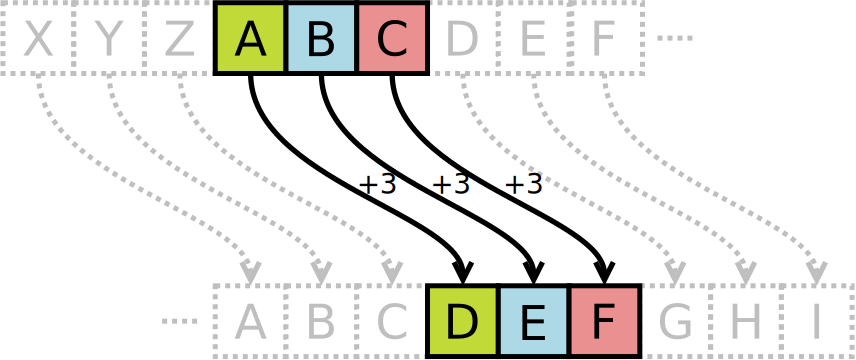
\includegraphics[scale=0.4]{eps/chiffrecesar}
  \end{center}
  \caption{Le chiffre de César}
  \label{fig:chiffrecesar}
\end{figure}

Au Moyen-âge, comme la plupart des sciences, la cryptologie n'évolue
presque pas, à part quelques exceptions au Moyen-Orient et en Asie
(dans le Kama-sutra, il est dit que les femmes doivent apprendre le
\emph{mlecchita-vikalpa} (l'art de l'écriture secrète) pour cacher
leurs liaisons.). Il faut donc attendre le XV\ieme siècle pour que la
cryptographie commence réellement à évoluer.

% Premières techniques de cryptographie
% Plus vieux document chiffré : un potier qui écrit sa recettes en
% enlevant des consonnes et en changeant l'orthographe des mots.
% En chine : stégano (papirus enroulé en boule recouvert de cire, avalé)
% première trace : vers 2000 av J.-C.
% Scytale -500 av J.-C. : == bâton de Plutarque.
% Spartiates, bâton rond, qu'on entoure d'un long et étroit morceau de
% parchemin. Une fois mis autour, on écrit le message dessus, puis on
% l'envoie au destinataire, qui possède une scytale de même diamètre,
% et qui déchiffre donc facilement le message. Fa
% Nabuchodonosor : -600 av J.-C. : 
% On rase le crâne d'un esclave, et une fois les cheveux repoussés, on
% l'envoie au destinataire, qui rase à nouveau les cheveux.
% Harpage qui envoie un message à Cyrus, il ouvre le ventre d'un
% lièvre pour y cacher une lettre, et l'envoya à Cyrus.
% Hebreux : Vieme av JC, atbash, chaque lettre est inversée A->Z,
% B->Y, ...

% ~-200 : premiers "vrais" systèmes cryptographiques : 
% caré de polybe, historiengrec : ~-150
% 1er siècle avant J.-C. : 
% code de césar utilisé dans l'armée romaine, réutilisé par la suite
% durant la guerre de sécession et l'armée russe en 1915 (rot13)

% Moyen age : quasi rien car sorcellerie, tout ça.

% Quasi rien jusqu'au XVieme 
%XV : encyclopédie de 14 volume écrite par un égyptien Abd Allah
%al-Qalashandi qui inclut une section sur la cryptologie. Elle y
%décrit des chiffres de substitution et de transposition.
% Leon Battista Alberti, humaniste italien de la renaissance,
% architecte, écrivain, philosophe et peintre. IMAGE
% écrit un essai parlant de cryptanalyse, avec
% l'analyse de fréquences des lettres en latin et italien. Invente
% aussi le cadran chiffrant, première méthode de chiffrement
% polyalphabétique.
% Cadran chiffrant : 2 disques contenant les lettres de l'alphabet, 
%dont un qui tourne (20 lettres chez Alberti, et le cadran faisait 24
%cases, JUW pas dans l'alphabet, et on omet H et K et Y (« qui ne sont pas
%indispensables », le deuxième cadran contient les 23 lettres latines
%+ le &) Après avoir chiffré 3 ou 4 lettres, on décale le disque, et
%on l'indique en notant de le message la lettre au dessus du k(lettre
%sur le petit).
% Notion de surchiffrement aussi. (à relire)

% 1518 : Jean trithème écrit Polygraphiae, premier livre imprimé sur
% la cryptologie, où il invente un chiffre stéganographique et ce qui
% deviendra par la suite le chiffre de Vigenère. voir la bonne partie

% Pendant certaines guerres en europe, les espagnols communiquaient
% via un chiffre, qu'ils changaient de temps en temps afin de troubler
% les gens qui pourraient essayer de le déchiffrer. Certaines lettres
% furent interceptés, et Henri IV chargea un géomètre, Viete, de
% trouver la clé de ces lettres. Il y réussit brillement, en
% comprenant le chiffre dans toutes ses formes possibles. La Cour
% d'Espagne, accusa le gouvernement français d'avoir recouru à des
% serciers, et voulait que Viete soit jugé comme un négromant en
% portant des plaintes à Rome. Il n'en fut rien mais à cette époque
% encore, c'était très dangereux d'être considéré comme un sorcier.

% Milieu du 16ème, Jérôme cardan invente le premier procédé autoclave,
% et une méthode stéganographique connue sous le nom de grille de
% cardan, où il cache le message dans une "grille de lettres", on
% retrouvera le message facilement 
